\documentclass[11pt]{article}
\usepackage{geometry}
\geometry{
	left=20mm,
	right=20mm,
	top=20mm,
	bottom=20mm,
	footskip=10mm
}

\usepackage{setspace} 
\usepackage{times}

%%%% either geometry or fullpage
%\usepackage{fullpage}

\singlespacing

\usepackage{graphicx,amssymb,setspace}
%\usepackage{algorithm,algorithmic}
%\usepackage[algoruled,linesnumbered,lined,boxed]{algorithm2e}
\usepackage{epsfig,tabularx,array,booktabs}
\usepackage{caption}
\usepackage{placeins}
\usepackage{multirow}
\usepackage{longtable}
\usepackage{hyperref}
\usepackage{subcaption}
\usepackage{tikz}
\usetikzlibrary{shapes}
\usetikzlibrary{arrows}
\usepackage{tabularx}
\tikzset{
	main node/.style={circle,draw,font=\small},
	rectangle/.style={font=\small}
}

\usepackage{xcolor}
\usepackage{url}
\usepackage{makeidx}
\usepackage{amsmath}
\usepackage{amsfonts}
\usepackage{caption}
\usepackage{multicol}
\usepackage{multirow}
\usepackage{graphicx}
\usepackage{float}
\usepackage{fancyhdr}
\usepackage{blindtext}
\usepackage{titlesec}
%\usepackage[backend=biber]{biblatex}

\newcommand{\figref}[1]{Figure~\ref{fig:#1}}

\titlespacing\section{0pt}{8pt plus 4pt minus 2pt}{4pt plus 2pt minus 2pt}
\titlespacing\subsection{0pt}{6pt plus 4pt minus 2pt}{3pt plus 2pt minus 2pt}
%\titlespacing\subsubsection{0pt}{12pt plus 4pt minus 2pt}{0pt plus 2pt minus 2pt}


\begin{document}

%\title{Research Statement\vspace{-0.5cm}}
%\author{Xudong Liu}
%\date{}
%
%\maketitle

\begingroup  
  \centering
  \huge Research Statement\\[0.25em]
  \large Xudong Liu\par
\endgroup


\section{Research Overview}
\noindent My research is rooted in preferences (i.e., 
preference modeling, learning and reasoning),
and social choice.
Preference modeling, learning and reasoning is a major research 
area in artificial intelligence (AI) and decision theory, and is closely related to the 
social choice theory considered by economists and political scientists. In my research I 
explore emerging connections between preferences in AI and social choice theory. 
Most of my research is on qualitative preference representation languages extending and combining
formalisms such as  
lexicographic preference trees (LP-trees) \cite{booth:learningLP}, 
answer-set optimization theories (ASO-theories) \cite{Brewka:ASO}, 
possibilistic logic \cite{dubois1991towards}, and 
conditional preference networks (CP-nets) \cite{boutilier2004cp};
on learning problems that aim at discovering qualitative preference 
models and predictive preference information from empirical data; and on
qualitative preference reasoning problems centered around preference optimization 
and strategy-proofness of preference aggregation methods.
Applications of my research include recommender systems, decision support tools,
multi-agent systems, and Internet trading and marketing platforms.

\section{Preliminaries}
\noindent The principle of my research concerns problems involving \textit{qualitative preferences}, that is,
simple and intuitive qualitative statements about \textit{preferred properties}
of alternatives.
These alternatives are described in terms of \textit{attributes} or \textit{issues}, 
each assuming values from some finite domain.
For instance, vacations can be described in terms of issues such as
\textit{activity} ($A$), \textit{destination} ($D$), \textit{time} ($T$), and \textit{transportation} ($R$),
where \textit{activity} has values \textit{water-sports} ($ws$) and \textit{hiking} ($h$),
\textit{destination} has values \textit{Florida} ($fl$) and \textit{Colorado} ($co$),
\textit{time} has values \textit{summer} ($s$) and \textit{winter} ($w$), and
\textit{transportation} has values \textit{car} ($c$) and \textit{plane} ($p$).
Thus, a sequence of attribute values, for example,
$\langle ws, fl, s, c \rangle$
describes a specific \textit{summer} vacation involving \textit{water-sports} 
in \textit{Florida} to which we travel by \textit{car}.
Spaces of alternatives of this type are referred to as \textit{combinatorial domains}.

The exponential size of the combinatorial domain leads to the infeasibility of
correctly putting precise numbers on the utility of specific choices; thus,
we turn to languages specifying preferences qualitatively.
The sheer number of alternatives in the combinatorial domain also makes it
impossible to enumerate from the most preferred to the least.
Consequently, my research focuses on designing \textit{concise} formalisms
in which qualitative preferences over such domains could be expressed
compactly and intuitively, and solving problems in preference learning and reasoning
in the context of these formalisms.

\begin{figure}[!ht]
\vspace{-0.3cm}
        \centering
  			\begin{subfigure}[b]{0.2\textwidth}
          \centering
          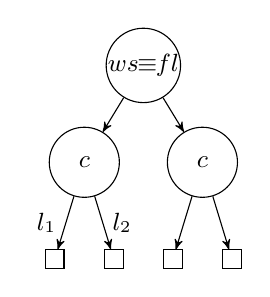
\begin{tikzpicture}[->,>=stealth',
            level/.style={sibling distance=1.5cm/#1, level distance=35pt}]
            \node [main node,inner sep=0pt] (1){$ws \!\! \equiv \!\! fl$}
              child {node [main node,inner sep=7pt] (2) {$c$}
                child {node [rectangle,draw] (3) {} edge from parent node[left] {\small{$l_1$}}}
                child {node [rectangle,draw] (4) {} edge from parent node[right] {\small{$l_2$}}}
                                }
              child {node [main node,inner sep=7pt] (5) {$c$}
                child {node [rectangle,draw] (6) {}
                                        }
                child {node [rectangle,draw] (7) {}
                                        }
              };
          \end{tikzpicture}
          \caption{\scriptsize Full P-tree \label{fig:pt_vac_full}}
        \end{subfigure}%
  			\begin{subfigure}[b]{0.25\textwidth}
          \centering
          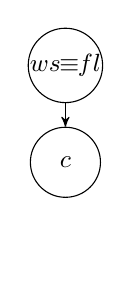
\begin{tikzpicture}[->,>=stealth',
            level/.style={sibling distance=2cm/#1, level distance=35pt}]
            \node [main node,inner sep=0pt] (1){$ws \!\! \equiv \!\! fl$}
              child {node [main node,inner sep=7pt] (2) {$c$}
                        child {node [rectangle] (4) {} edge from parent[draw=none]}
                                };
          \end{tikzpicture}
          \caption{\scriptsize Compact P-tree \label{fig:pt_vac_compact}}
        \end{subfigure}%
				\begin{subfigure}[b]{0.35\textwidth}
          \centering
				  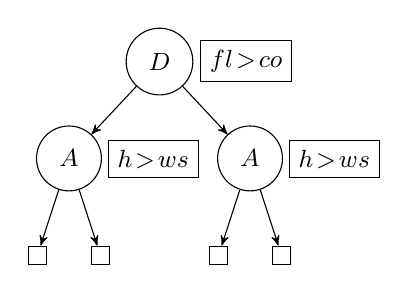
\begin{tikzpicture}[->,>=stealth'
				    ,level 1/.style={sibling distance=2.3cm}
				    ,level 2/.style={sibling distance=0.8cm}
						,level/.style={level distance=35pt}
					]
				    \node [main node,inner sep=5pt] (1){$D$}
				      child {node [main node,inner sep=5pt] (2) {$A$}
				        child {node [rectangle,draw] (3) {}}
				        child {node [rectangle,draw] (4) {}
				          child {node [rectangle,draw] at (2.65,3.7) {$fl\! >\! co$} edge from parent[draw=none]}
				          child {node [rectangle,draw] at (0.67,2.45) {$h\! >\! ws$} edge from parent[draw=none]}
				          child {node [rectangle,draw] at (2.17,2.45) {$h\! >\! ws$} edge from parent[draw=none]}
				        }
				      }
				      child {node [main node,inner sep=5pt] (5) {$A$}
				      child {node [rectangle,draw] (6) {}}
				        child {node [rectangle,draw] (7) {}}
				      };
				  \end{tikzpicture}
					\vspace{-1cm}
					\caption{\scriptsize Full PLP-tree \label{fig:plpt-full}}
				\end{subfigure}%
				\begin{subfigure}[b]{0.25\textwidth}
          \centering
          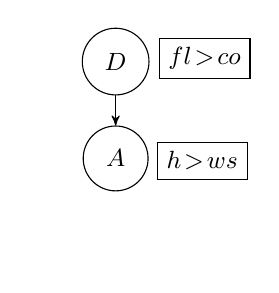
\begin{tikzpicture}[->,>=stealth',
            level/.style={sibling distance=2cm/#1, level distance=35pt}]
            \node [main node,inner sep=5pt] (1){$D$}
              child {node [main node,inner sep=5pt] (2) {$A$}
                child {node [rectangle] (4) {} edge from parent[draw=none]}
				      		child {node [rectangle,draw] at (1.13,2.5) {$fl\! >\! co$} edge from parent[draw=none]}
				      		child {node [rectangle,draw] at (0.1,1.2) {$h\! >\! ws$} edge from parent[draw=none]}
                                };
          \end{tikzpicture}
					\vspace{0.1cm}
					\caption{\scriptsize Compact PLP-tree \label{fig:plpt-col}}
				\end{subfigure}
  \caption{P-trees and PLP-trees on vacations}
  \label{fig:pt_vac}
\vspace{-0.3cm}
\end{figure} 
One of such preference systems, \textit{preference trees} (P-trees), was
introduced by Fraser \cite{fraser1994}, and formally defined in my work \cite{wsh/mpref14/LiuT,LiuT:PT}.
I will illustrate this formalism with preferences over the vacation domain.
Let us say that the most important property for an agent concerns activity and destination.
She prefers vacations with water sports
in Florida or hiking in Colorado over the other options. This
preference is described as an equivalence formula $ws \equiv fl$.
Within each of the two groups of vacations (satisfying the
formula and not satisfying the formula), driving ($c$) is the preferred transportation mode.
These preference statements are described as a P-tree in \figref{pt_vac_full}.
Clearly, the P-tree partitions the vacations into four clusters, denoted by
the leaves, with the leftmost representing the set of most preferred vacations
satisfying the formulas $ws \equiv fl$ and $c$.
Thus, the alternative $\langle h, co, s, c \rangle$ is better than
vacation $\langle ws, fl, s, p\rangle$, 
because the former descends to leaf $l_1$ and the latter descends to leaf $l_2$, and $l_1$
precedes $l_2$ in the order of leaves.
Since the subtrees of the root are the same and leaves can be omitted in \figref{pt_vac_full},
we can collapse the full tree to its \textit{compact} version in \figref{pt_vac_compact}.
Compactness of preference models is
crucial in studying problems in preference learning and reasoning.

I introduced the preference formalism of \textit{partial lexicographic preference trees},
or PLP-trees \cite{LiuT:Learn_PLPTrees}, where nodes in the tree are labeled not by a formula 
but by an attribute and a total ordering of the values of the attribute.
To illustrate PLP-trees, let us consider again preferences over vacations.
As shown in \figref{plpt-full}, our agent puts \textit{destination} as the most important attribute on which
she prefers \textit{Florida}.
Similarly as before, she next considers \textit{activity} and prefers 
\textit{hiking} for both \textit{Florida} and \textit{Colorado} vacations.
Like the above P-tree, this full PLP-tree induces a total preorder of four 
clusters of equivalent alternatives as the box-labeled leaves, and it is collapsed to a
much more compact one in \figref{plpt-col}, where 
preferences on all attributes are \textit{unconditional}.
I have shown that PLP-trees are special cases of 
P-trees but more general than the restrictive LP-trees.
Studying learning and reasoning problems for PLP-trees will contribute
to the most general setting of P-trees.


\section{Current and Ongoing Research}
\noindent My work, in collaboration with professors and colleagues in our department,
has resulted in refereed publications at premier venues on preference modeling \cite{wsh/mpref14/LiuT,LiuT:PT}, learning
\cite{LiuT:Learn_PLPTrees} and reasoning \cite{LiuT:LPT_ASP_EA,LiuT:LPT_ASP,Spradling}.
My thesis abstract was also published at a leading conference on decision theory \cite{Liu:TA}.

\subsection{Preference modeling}
\noindent We formally defined the language of P-trees,
studied the relationship between P-trees and other existing preference languages, and
showed that P-trees extend  
LP-trees, possibilistic logic theories, and ASO-rules\cite{wsh/mpref14/LiuT,LiuT:PT}.
Moreover, we established computational complexity results of commonly considered decision
problems in the setting of P-trees, such as \textit{dominance testing} 
(asking if an alternative is preferred to another given the preferences),
\textit{optimality testing} (deciding if an alternative is optimal given the preferences), and
\textit{optimality testing w.r.t a property} (determining if there exists an optimal alternative
satisfying a given property).

\subsection{Preference Learning and Approximation}
\smallskip \noindent \textbf{Preference Learning \ }
We introduced the formalism of PLP-trees, a novel formalism for lexicographic preference models,
also a subclass of P-trees, over combinatorial domains of alternatives \cite{LiuT:Learn_PLPTrees}.
For PLP-trees we investigated the problem of \textit{passive learning},
that is, the problem of learning preference models given a set of
pairwise preferences between alternatives, called \textit{training examples}, provided by the user upfront.
Specifically, we studied how to learn (i) a PLP-tree, preferably of a small size, 
consistent with a dataset of examples, and (ii) a PLP-tree correctly
ordering as many of the examples as possible in case
of inconsistency. We established complexity results
of these problems and, in each case where the problem
is in the class P, proposed a polynomial time algorithm.

Continuing this research direction,
I am working on generalization of my results on learning PLP-trees to the case of P-trees.
I am also designing and implementing algorithms to learn, from both synthetic and real-world datasets, preferences
described in formalisms
of LP-trees, PLP-trees and P-trees for both passive learning and active learning.
To facilitate the preference learning process, I am developing datasets of examples from existing
learning datasets from sources such as the Library for Preferences (\url{http://www.preflib.org/}),
the Preference Learning Site (\url{http://www.preference-learning.org/}), 
and the UCI Machine Learning Repository (\url{http://archive.ics.uci.edu/ml/}).
To evaluate our own models, I plan to
apply machine learning methods to obtain preferences from these developed datasets.

\smallskip \noindent \textbf{Preference Approximation \ }
Some models, e.g., CP-nets, of preference orders do not support effective reasoning.
However, learning can provide a way to circumvent the difficulty of high computational complexity
of reasoning tasks, such as \textit{dominance testing}.
Compared to the formalism of CP-nets, P-trees are more intuitive
for representing preferences over combinatorial domains, and are easier to reason with.
Thus, I am studying the hidden relations between the two systems, searching for 
algorithms to approximate
CP-nets using P-trees learned from examples consistent with the CP-net.
This might open a way to more effective reasoning with hard preference languages.

\subsection{Preference Reasoning}
\smallskip \noindent \textbf{Preference aggregation  \ }
We investigated two preference-aggregation 
problems, the \emph{winner} problem, computing the winning alternative in an election,
and the \emph{evaluation} problem, computing an alternative scoring at least above
some threshold in an election,
based on \textit{positional scoring rules} (such as $k$-approval and Borda) 
when preferences are represented as LP-trees\cite{LiuT:LPT_ASP}. 
We obtained new computational complexity results of these two problems and
provided computational methods to model and solve the problems in two programming formalisms, 
answer set programming (ASP) and weighted partial maximum satisfiability (WPM).
To support experimentation, we designed methods
to generate LP-tree votes randomly and presented experimental results
with ASP and WPM solvers.

\smallskip \noindent \textbf{Preferences in game theory and planning  \ }
We introduced a new variant of hedonic coalition formation
games in which agents have two levels of preference on their own coalitions:
preference on the set of ``roles" that make up the coalition, and
preference on their own role within the coalition\cite{Spradling}. 
We then defined and studied several stability
notions and optimization problems for this model.
Applying theories into practical problem solving, I designed and developed software modules
for representing and reasoning about user constraints and preferences in a trip planning
setting.

\smallskip \noindent \textbf{Preference misrepresentation  \ }
I am studying problems related to vulnerability of collective decisions under misrepresentation of preferences
specified over combinatorial domains.
Take the \textit{coalitional manipulation problem} as an example.
This problem asks to decide if a small coalition set of manipulative
voters can make some candidate a winner.
I will examine other positional scoring rules, as well as
some comparison-based (e.g., the Copeland, Simpson and Maximin rules) and 
distance-based voting (e.g., the Kemeny and Dodgson rules) systems, for LP-trees,
and extend these results to elections over complicated domains to more general cases.

\section{Future Research Objectives}
\noindent My long-term research goal is to study computational problems related to preferences, and 
develop applications that help people or software agents make better decisions.
Particularly, I intend to embed theories and practices on preferences into areas including
data science, and automated planning and scheduling.

\smallskip \noindent \textbf{Data science \  } Discovering preference 
models from large data sets and reasoning about them 
can be of great value when decisions need to be customized for individual users.
For instance, e-Commerce companies want to make quality marketing decisions
on what customers would be interested in purchasing at a future time.
I propose to introduce contextual information and human-in-the-loop into existing learning methods
(e.g., collaborative filtering and content-based filtering used in recommender systems), 
in order to provide context-aware and user-centered predictions.
I also plan to build preferential data sets and develop predictive systems, with collaborators
or sponsors from fields 
such as machine learning, computer vision, psychology, cognitive science, and behavioral science.

\smallskip \noindent \textbf{Automated planning and scheduling \  }
In planning and scheduling, constraints and preferences of agents may be more faceted than simply
``fastest" or ``cheapest."
Expanding my research work at Palo Alto Research Center,
I propose to design mathematical languages allowing
intuitive representations of these individual accommodations. 
Furthermore, I intend to implement systems
that automate the acquisition of user constraints and preferences, and the computation of optimal plans or schedules 
based on these user-specific information.
This line of research potentially promotes collaboration with researchers of expertise in
travel scheduling, manufacturing, and traffic control.

As my research is highly applicable in practice, it could attract both undergraduate and graduate students to
get involved in these research directions.
I expect to attract companies and research institutes
for real-world data and exterior funding opportunities
to support my research.

\bibliographystyle{plain}
{\bibliography{RS_Xudong_Liu}}


\end{document}
